As the Internet of Things and mobile devices have become ubiquitous and 
increasingly powerful, so has demand on their capabilities. Users often want 
both great performance and great battery life out of numerous devices. The 
introduction of Asymmetric Multicore Processors (AMPs) like ARM's big.LITTLE 
technology has helped meet these demands as the big cores can be switched off 
until needed, thereby saving power. This has led to the concept and management  
of ``dark silicon'' -- processing elements which have been switched off to save 
energy.

As with most changes, it takes a bit of time for the software to catch up. The 
Linux Scheduler had to be redesigned in the 2000s in order to work better with 
Multicore Processors, and even after the redesign, improvements continued to 
emerge. Recently, there has been interest in making schedulers energy aware. 
Since the scheduler manages which tasks run when and on what CPUs, there is an 
idea that improvements could be made on existing systems if the scheduler was 
aware of the different types of cores and the energy they use. By having this 
insight, it could manage the Dynamic Voltage and Frequency Scaling (DVFS) on 
the cores with much finer control than current approaches, potentially leading 
to great energy savings at a low performance cost.

The ARM big.LITTLE architecture provides special registers and hardware known 
as Performance Monitoring Units (PMUs). These allow software to efficiently 
keep track of how many times certain events happen on the hardware. Although 
many PMU events (and hence measurements) are supported, typically only 5-7 can 
be retrieved at a time. This leads to an interesting problem in the form of 
which ones to prioritise. With the right combination of PMU events and a model 
built to represent how they affect performance and energy, the scheduler could 
be able to make intelligent decisions based on the dynamic monitoring of both 
task and harware performance. As ARM big.LITTLE, energy awareness, and PMUs are 
only recently beginning to gain attention in the literature, this leaves many 
interesting and highly applicable research areas open.

In this project, I explore how to use the gem5 simulator to model DVFS and 
power consumption in big.LITTLE systems. I then use it to explore if 
predictions based on existing PMU data obtained from a stock configuration can 
be used to correctly predict the optimal big.LITTLE configuration to run the 
program on. I find that although gem5 can be challenging to use, the simulations
are possible and even limited data can be used to create promising models for 
predicting the optimal configuration. This is promising for further research 
into the area.
\begin{figure}[H]
    \centering
    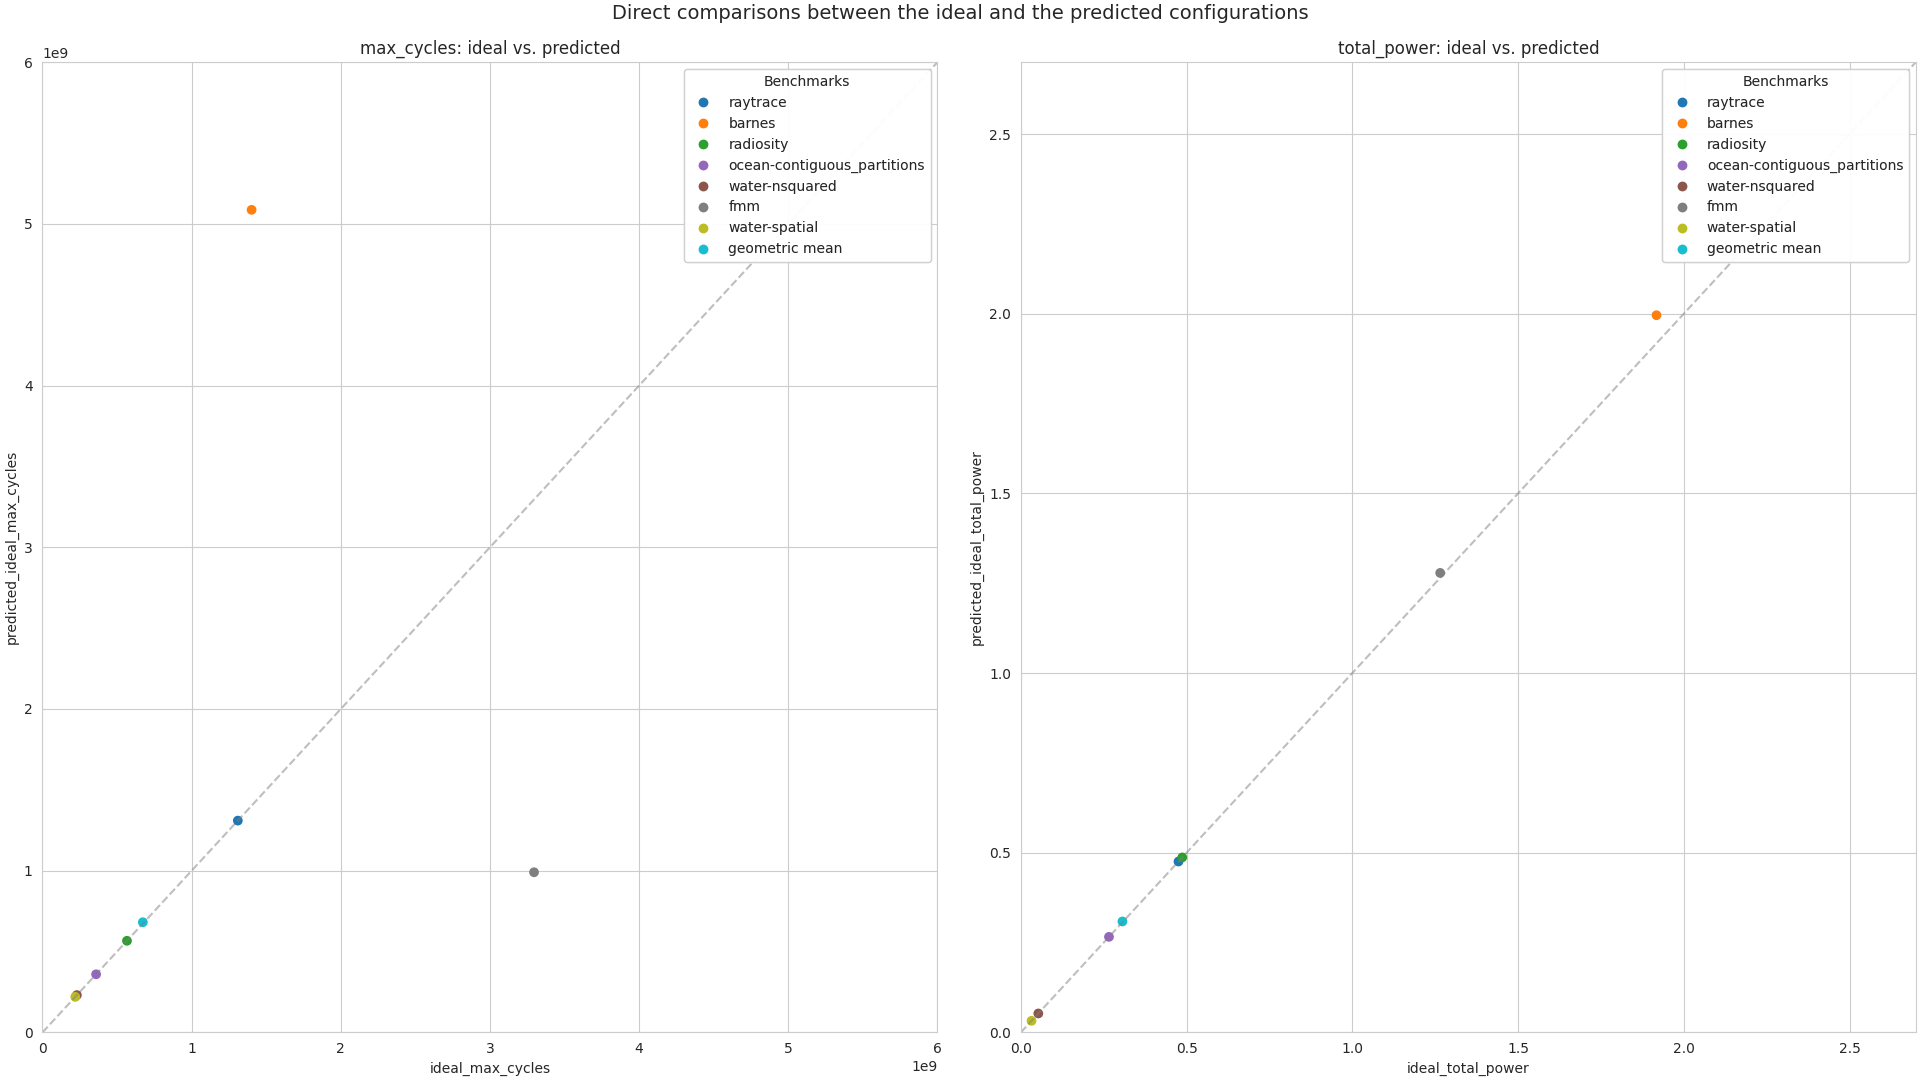
\includegraphics[width=\textwidth]{result-plots/stock-2b2L/system-scatter.png}
    \caption{Initial results based on data obtained from gem5 seems highly
             promising in terms of the use of PMUs in scheduling}
\end{figure}
